\documentclass{article}[11pt]
\usepackage[utf8]{inputenc}
\usepackage{graphicx} 
\linespread{1.5}
\usepackage{lineno}
\linenumbers
\usepackage[a4paper, total={6in, 8in}]{geometry}
\usepackage[font=small,labelfont=bf]{caption}

\title{Evaluating microbial growth patterns using mathmatical models: Polynomial quadratic vs logistic}
\author{Kate Griffin, Imperial College London}
\date{December 2021\\Word Count: 2324}


\begin{document}

\maketitle
\newpage
\tableofcontents
\newpage
\begin{flushleft}
	
\section{Abstract}
Mathematical models can be powerful tools in evaluating questions in biology and ecology. One important application is evaluating the growth of microbes over time. Bacterial follow a sigmodial growth pattern, whereby an exponential growth phase commences after a lag period. Existing models can describe this pattern, and make predictions about their growth based on a suite of given parameters. Biological models may be considered as being on a spectrum between phenomenological to mechanistic approaches, based on the scope of their parameters. Although mechanistic models may be more robust, they are not necessarily better at describing real biological processes, such as microbial growth. In my analysis I investigate whether a simple quadratic model or a more mechanistic model (a modified logistic model) was better suited at describing the growth pattern of microbes. The data used in this analysis included forty-five species of microbes grown on eighteen different media, data for which was collected across the world. My analysis found that the quadratic model was better at describing the relationship between population size/abundance and time. I will discuss the limitations and applications of this study. 


\newpage
\section{Introduction}

Food spoilage may be defined as any change in a food product which deems it unsuitable for consumption by a consumer \cite{bae2014growth}. The most common cause of food spoilage is that caused by microbes, which can alter a food item’s flavour, smell, texture and taste \cite{bae2014growth}. The surfaces of food products are often nutrient rich and, in combination with suitable environmental conditions, this can facilitate the growth of biofilms \cite{bae2014growth}. In the food industry, predicting microbial growth may be useful in evaluating risk and shelf life of perishable goods \cite{huang2013optimization}\cite{bae2014growth}\cite{zwietering1990modeling}. Microbial growth rates may be measured by plotting population density against time on a graph and fitting a straight line through the exponential growth phase. The slope of this line represents the maximum growth rate (r max). In recent years, predictive microbiologists use mathematical models which can describe the growth of microorganisms along the sigmoidal bacterial growth curve. Such models include the Gompertz, Logistic, Baranyi and Buchanan models\cite{huang2013optimization}.
\linebreak

The growth of a bacteria in batch culture may be divided into five main phases based on the slope of its growth curve \cite{rolfe2012lag}\cite{huang2013optimization}\cite{finkel2006long}\cite{zwietering1990modeling}. The first phase is the lag phase, where bacteria adapt themselves in preparation for their growth. During this phase, a number of genes are activated, including those involved in the uptake of nutrients, DNA repair, RNA processing, cell division and other biomolecular processes. The next phase is the exponential growth phase, where cell division occurs at a constant rate following a geometric progression. Once carrying capacity of the environment (i.e., growing media) has been reached, the stationary phase commences. During this phase, bacteria stop replicating. The next phase is the death phase, which occurs when the bacterial cells lose viability. The last stage is the long-term stationary phase,  where bacteria can remain for long periods of time without nutrients \cite{finkel2006long}.
\linebreak


Ecological and evolutionary models may be considered as a spectrum between phenomenological to mechanistic methods \cite{white2019should}. Models may be described as mechanistic if they include a number of parameters with biological definitions, which may be measured independently of the observed data \cite{transtrum2016bridging}\cite{white2019should}. In comparison, phenomenological models (e.g., cubic and quadratic polynomial models) measure a hypothesised relationship between two or more variables in a dataset, which can be fitted to the data \cite{white2019should}. When applied to measure population growth, the logistic model takes the carrying capacity of the environment into account. It demonstrates that the per capita growth rate decreases as population density increases \cite{stefan2012mathematical}. This is because populations grow exponentially while their population size is low and resources are not limiting, and then slows down as the population becomes so large that resources become limited (i.e., the Malthusian principle). The logistic model may be considered a mechanistic model when modelling population size, as it can be modified to include parameters which have biological meaning.
\linebreak


Although mechanistic models are more robust than phenomenological models, they are not necessarily more valuable in making predictions \cite{white2019should}. Mechanistic models are particularly suitable for analysing populations when predictions outside of the known set of parameters is required and there is also enough existing data to make a priori estimates of its parameters \cite{white2019should}. When a biological system or processes can be explained by relatively few variables, a simpler model with fewer parameters may be more useful \cite{transtrum2016bridging}.The aim of my analysis is to address the question as to whether phenomenological models or logistic models are better for modelling population growth in microbial batch cultures. In my analysis I will be comparing a quadratic polynomial model to a mechanistic logistic model in predicting the change in microbe abundance over time.

\newpage
\section{Methods}
\subsection{Preparing the data}
The dataset used in this analysis contains measurements of biomass/number of cells of forty-five species of microbes grown on eighteen different media over time. The data was collected from ten different studies across the world. Field names are defined in the metadata file. The two main variables I will be comparing are “PopBio” (abundance) and “Time”. Single population growth curves were identified as unique combinations of temperature, growing media, species and citation. These unique IDs were saved in a new column and used to subset the data. The data was wrangled in Python. Firstly, the data was checked for NA values as well as negative values for PopBio and Time. Rows which contained negative values were deleted. There were no NA values found in the dataset. The wrangled data with the unique ID column was then saved as a .csv file.
\linebreak

\subsection{Fitting the models}
The models were defined and ran in R. The models were fit in order to find their estimated parameters. AIC and BIC were then calculated to find the fit of the model parameters to the observed data. The first model fitted was the polynomial quadratic model, the equation for which is:

\[B = B\textsubscript{0}+B\textsubscript{1}x+B\textsubscript{2}x\textsuperscript{2}\]

where x represents an independent variable, which in this analysis is time. B\textsubscript{0}, B\textsubscript{1}, B\textsubscript{2} represents the parameters, i.e., the coefficients of the equation (respectively: the quadratic coefficient, the linear coefficient and the constant or term). Once the model was defined, it was ran on each subset of data. The AIC and BIC were calculated and saved.
\linebreak

The next model to be fit was the logistic model, the classic  equation for which is:

\[Nt = \frac{N\textsubscript{0} K e\textsuperscript{rt}}{K + N\textsubscript{0} (e\textsuperscript{rt} - 1)}\]

The three parameters defined in the model are: r (maximum growth rate, also known as R max), K (carrying capacity) and N\textsubscript{0} (initial population). Nt represents the population size at time t, and No is the initial population size. As with the quadratic model, the model was fit to find its parameters and ran on each subset. The initial population size was set as the lowest population size value for each subset, and the K starting value was set to the maximum population size. A random value for the initial r max value (0.0001) was selected. AIC and BIC were calculated to evaluate the fit.

\subsection{Plotting and analysis}

The difference in AIC between the quadratic and the logistic model was calculated for each subset. If the absolute difference was greater than 2, then the model with the smaller AIC value was selected as the better model. I created a tally of the models selected for each subset to compare which model was selected more often based on AIC. BIC was also then compared using the same method as AIC. Plots were created to visualise the fit of the models against the observed data as well as the tally of the most suitable model.

\subsection{Computing tools}
In this analysis, I used Python to load, analyse and wrangle the data. I used Pandas to load in the microbial data as a data frame. Pandas is an open source library, built upon  Numpy, which is used to handle numeric data in tabular form. Pandas provides a flexible and intuitive way to analyse and understand data, and is good at handling large datasets. Pandas was used to create unique IDs, which were then used to subset the data. Pandas was also used to create a new column to the dataframe, which the ID values were added to. The models were fit and ran on each subset of data using R. In order to perform a non-linear least-squares analysis, minpack.lm was installed. The "plyr" package (dlply and ldply) was also used to apply the quadratic model to each subset of data and to calculate AIC and BIC. The results were visualised in R, using ggplot to create plots for the results of the AIC and BIC analysis as well as plots for comparing the fit of the models to the observed data. I chose R to visualise the data as it offers a number of useful inbuilt functions and libraries (such as ggplot), and it is also a flexible and user friendly programming language. LaTeX was used to produce a .pdf file of the final report, as it good at handling mathematical notation and allows for easy formatting of citations and bibliography. A bash shell script was produced to run each script together. 


\newpage
\section{Results}
The quadratic and logistic model achieved fits on each of the 285 subsets. Plots were made to compare the predicted values of the models aginst the observed data [Fig.1][Fig.2]

%\linebreak

\begin{figure}[h]
	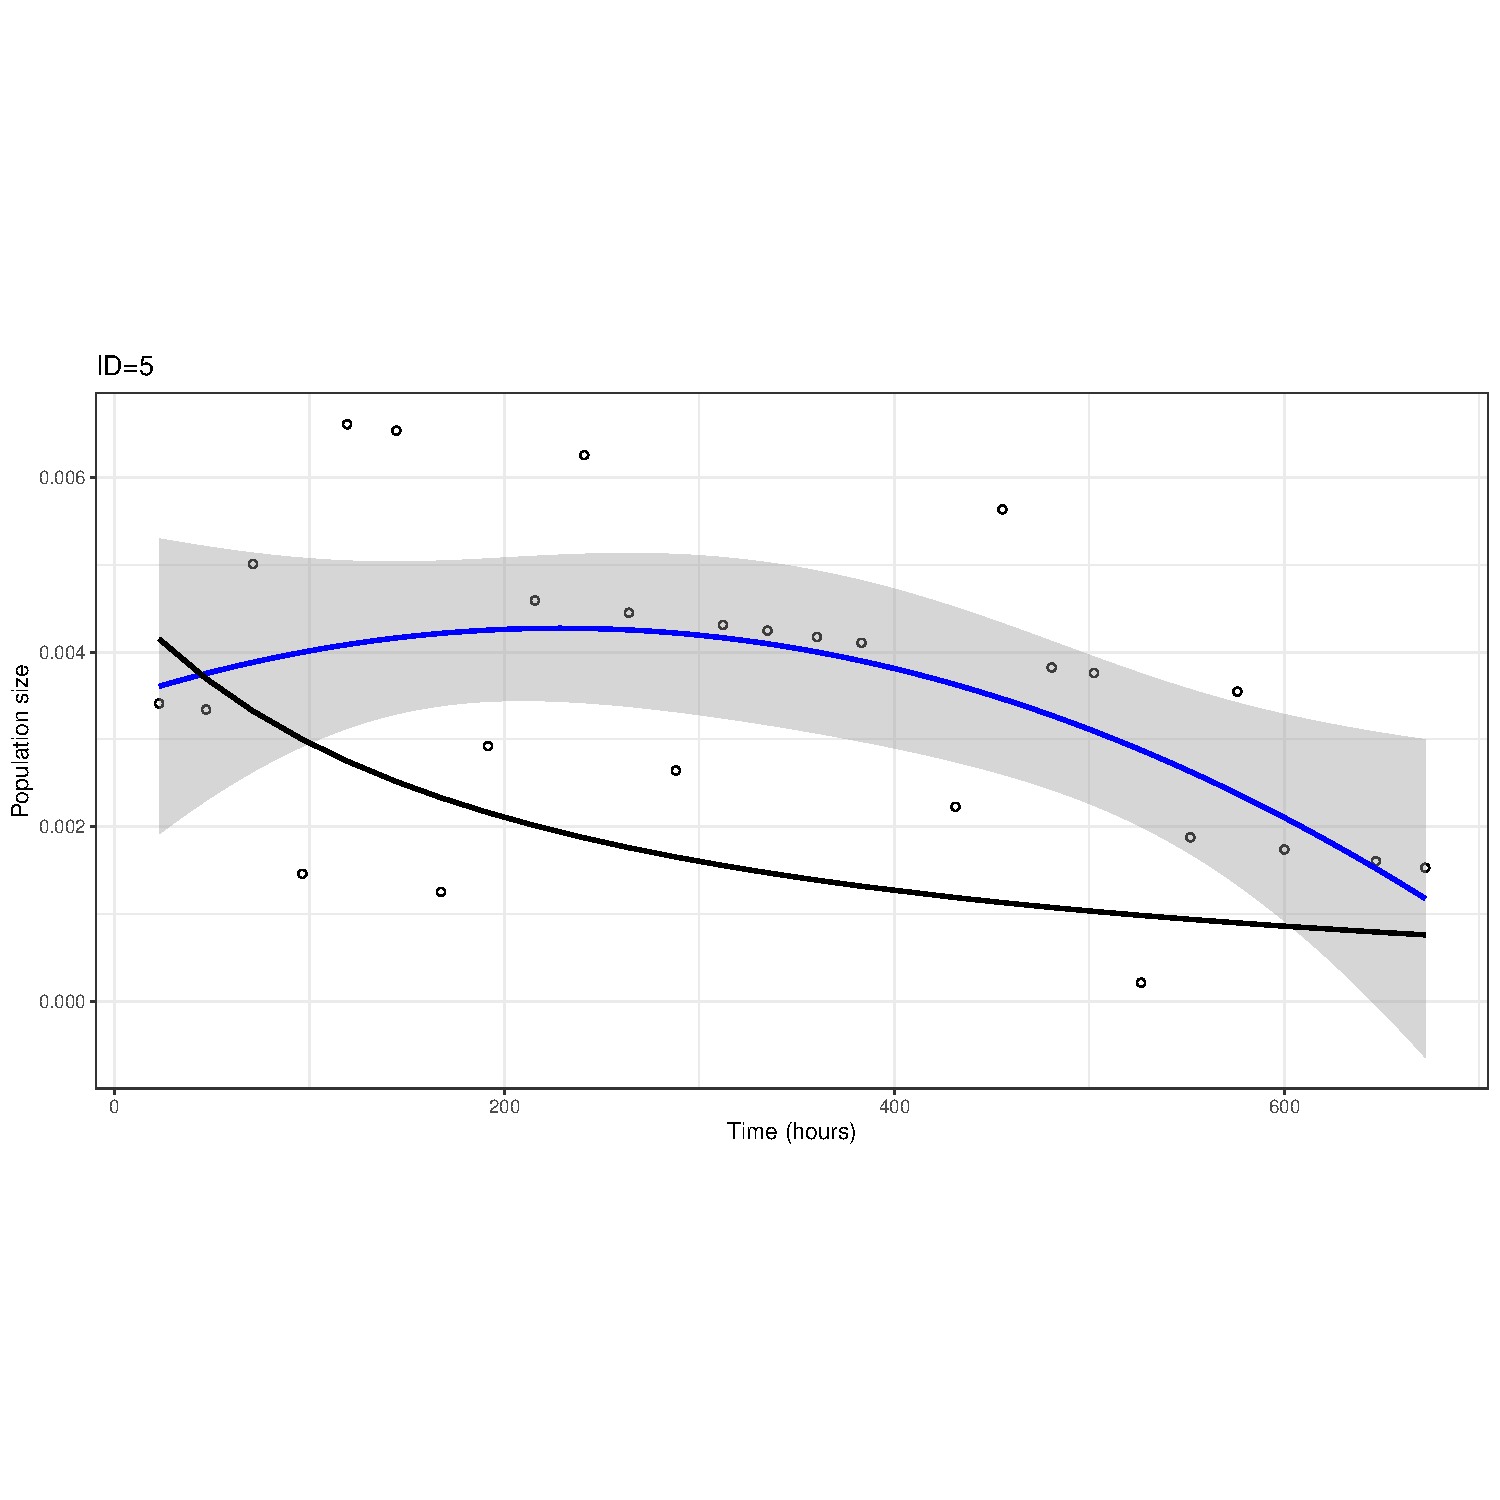
\includegraphics[width=12cm,height=12cm,keepaspectratio]{plot5.pdf}
	\centering
	\caption{Graph comparing the observed data to the predicted parameters of the models agaist the observed data for subset number 5. The blue line represents the quadratic model's predictions and the black line represents the logistic model's predictions. The points on the graph represent the data points}
\end{figure}

%\linebreak

\begin{figure}[h]
	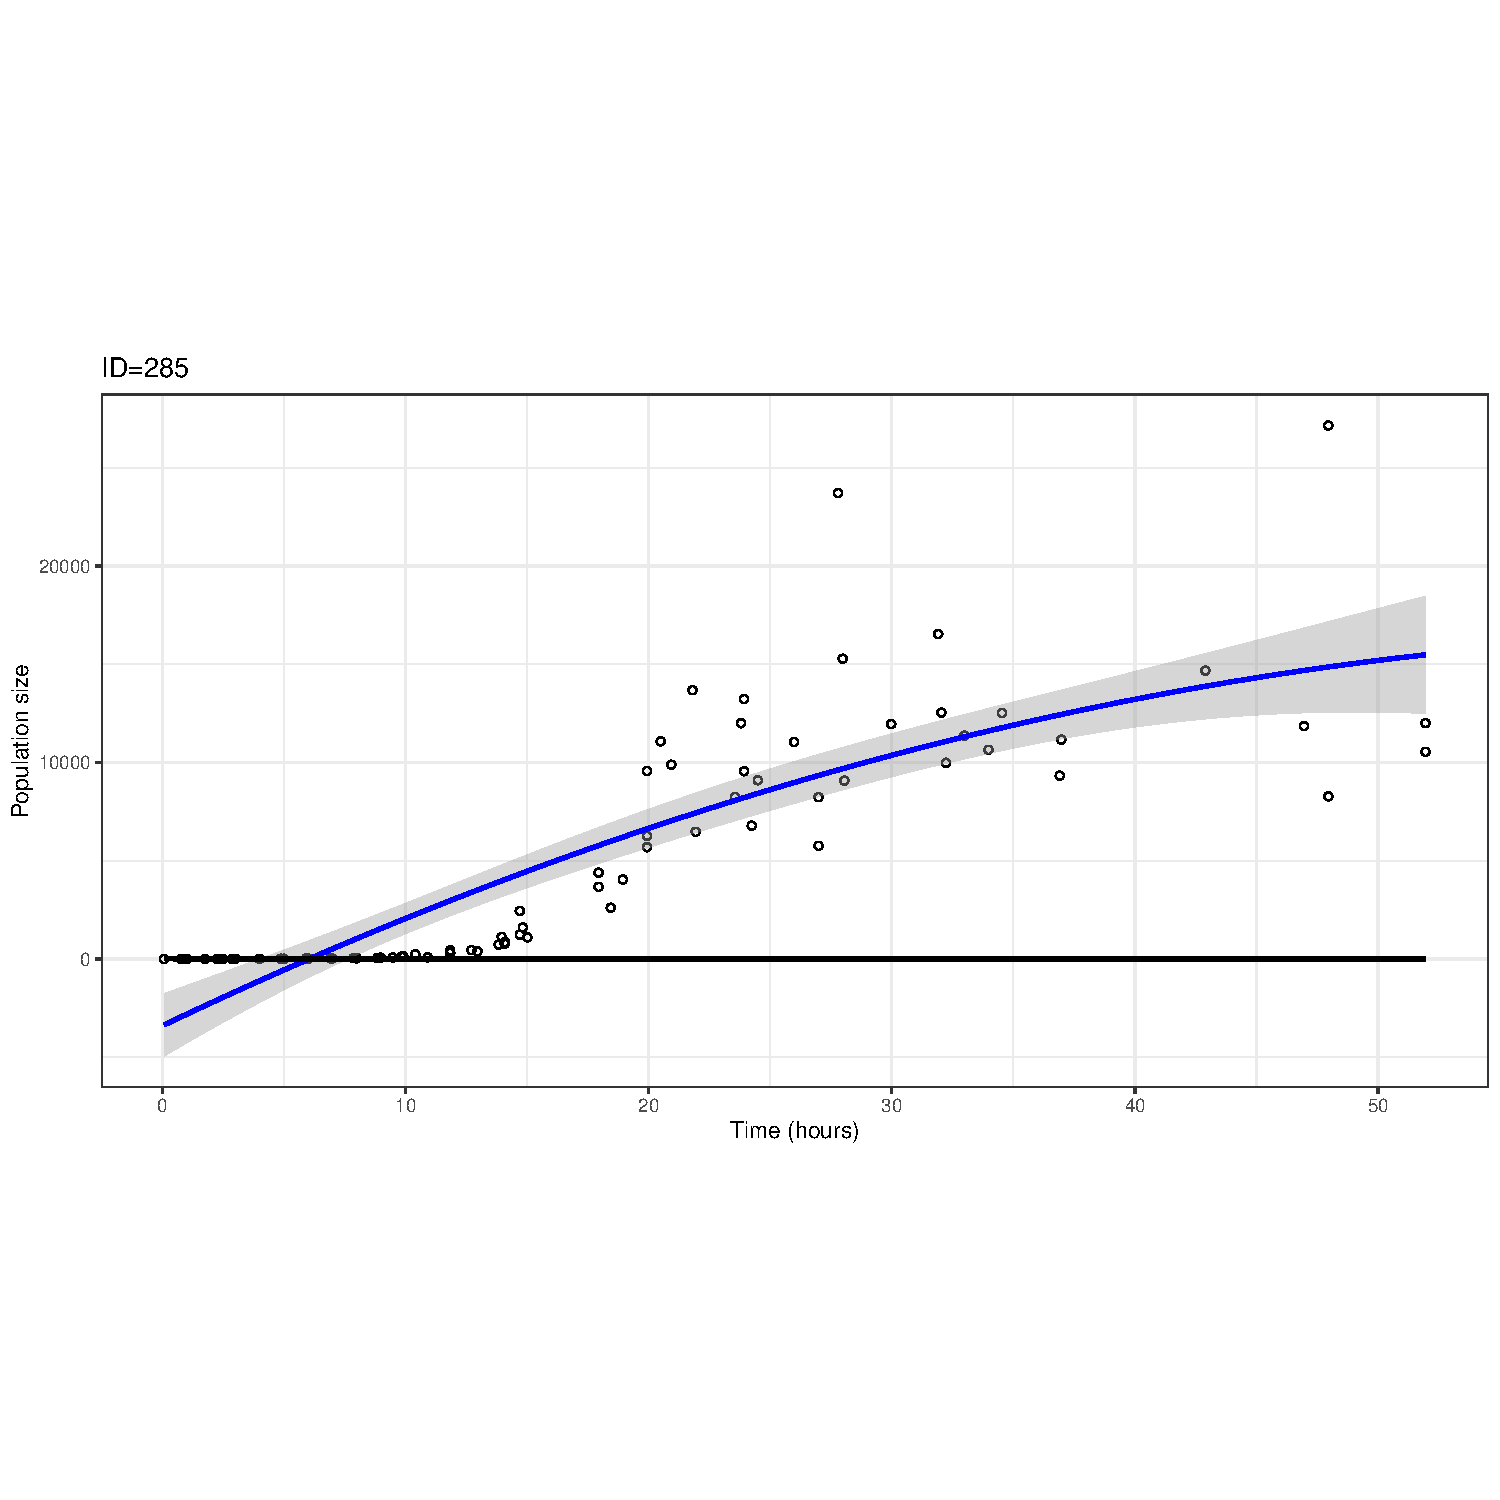
\includegraphics[width=12cm,height=12cm,keepaspectratio]{plot285.pdf}
	\centering
	\caption{Graph comparing the observed data to the predicted parameters of the models agaist the observed data for subset number 285. The blue line represents the quadratic model's predictions and the black line represents the logistic model's predictions. The points on the graph represent the data points}
\end{figure}
%\linebreak

The results of the AIC and BIC analysis suggested that the quadratic model was better at predicting the growth of microbes more often than the logistic model. The quadratic model was determined as the better model for 217 out of the 285 subsets for both the AIC and BIC analysis[Fig.3, Table.1]. The logistic model, in comparison, was only determined as the beter model for 48 out of the 285 subsets for both AIC and BIC comparisons [Fig.1, Fig.2].
\linebreak

\begin{figure}[h]
	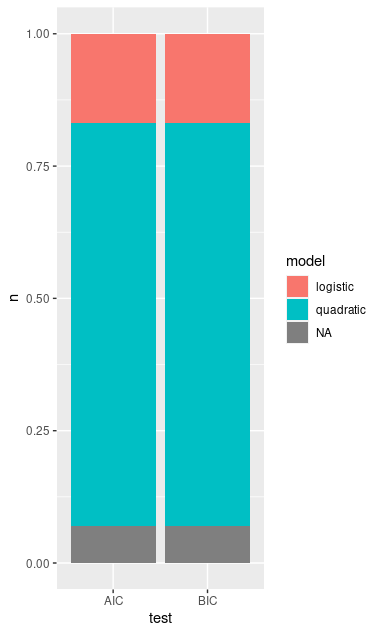
\includegraphics[width=12cm,height=12cm,keepaspectratio]{best_model.png}
	\centering
	\caption{Bar chart showing how often the logistic or quadratic model was selected as the best model for each subset of data, based on AIC and BIC}
\end{figure}

\begin{table}
	\centering
	\begin{tabular}{||c c c c||} 
		\hline
		Test & Selected model & n & \\ [0.5ex] 
		\hline\hline
		AIC & Logistic & 48 & \\ 
		\hline
		AIC & Quadratic & 217 &\\
		\hline
		AIC & NA & 20 & \\
		\hline
		BIC & Logistic & 48& \\
		\hline
		BIC & Quadratic & 217 & \\ [1ex] 
		\hline
		BIC & NA & 20 & \\ [1ex] 
		\hline
	\end{tabular}
	\caption{Tally of the number of times each model was selected as the better model for every subset of data (n) \label{long}}
\end{table}
\clearpage

\section{Discussion}
The aim of my analysis was to fit a logistic model (quadratic polynomial) and a mechanistic model (logistic) to an empirical dataset to evaluate which model fit the data best. My analysis found that the quadratic model was better than the logistic model at describing the bacterial growth curve on 217 of the 285 subsets in the Logistic Growth dataset. In comparison, the logistic model fit the data better than the quadratic model on only 48 out of the 285 subsets. These results may suggest that a more simple phenomenological model may have been better suited on analysing this particular dataset. This may be because phenomenological models have fewer parameters, and therefore there is less uncertainty in their results. \cite{white2019should}\cite{transtrum2016bridging}
\linebreak


The sample size of the data may have lead to increased uncertainty in the results, as some of the subsets had few data points (equal to or less than the number of parameters of the logistic model, i.e., 3) \cite{white2019should}. It may be beneficial if future lab estimates of population growth were sure to include enough observations so that commonly used mechanistic models may be sufficiently fit to the data (i.e., more than the number of  model parameters). Another limitation of this analysis is that the logistic model was ran with a random starting value. A more statistically sound approach may be to perform a rolling regression in order to find r max for each subset, and then to sample randomly from a normal distribution (where r max is the mean). Error may have been introduced while trying to define the parameters of the model. This analysis measured the relationship between bacteria growth and time for the same species and under similar environmental conditions. A future approach could be to analyse the effect of other co-variants (for example, the effect of temperature or growing medium) on model selection (i.e, different models may be better on certain media or temperatures). 
\linebreak

Although the quadratic model fit the data better in this study, there are still limitations of phenomenological models when describing the relationship between bacterial growth and time. This is because phenomenological models lack parameters with real biological meaning. Mechanistic models, in comparison, can describe real systems or processes, and can take measurements which can be applied in further studies, e.g., calculating carrying capacity \cite{white2019should}\cite{o1989multiple}. Ecological and evolutionary models have a wide variety of real world applications, including in resource management, planning ecological and environmental policies and environmental impact assessments \cite{o1989multiple}. The predictive power of models makes them particularly powerful tools in investigating biological questions, such as evaluating ecosystem functioning or understanding the mechanisms of disease pathophysiology and related drug action \cite{o1989multiple}\cite{brown2018applications}. For this reason, there is a significant value in evaluating and comparing existing ecological and biological models. 




\clearpage
\bibliographystyle{plain}

\bibliography{FirstBiblio}

\end{flushleft}
\end{document}
